\documentclass{article}

\usepackage[final]{nips_2017}

\usepackage[utf8]{inputenc} % allow utf-8 input
\usepackage[T1]{fontenc}    % use 8-bit T1 fonts
\usepackage{hyperref}       % hyperlinks
\usepackage{url}            % simple URL typesetting
\usepackage{booktabs}       % professional-quality tables
\usepackage{amsfonts}       % blackboard math symbols
\usepackage{nicefrac}       % compact symbols for 1/2, etc.
\usepackage{microtype}      % microtypography
\usepackage{authblk}
\usepackage{graphicx}
\usepackage{float}


\title{The Effects of Different Sampling Techniques on the SoundCloud Network}

\author{
	Josiah Buxton \hspace{45pt} Christopher Godley\\
	Department of Computer Science\\
	University of Colorado Boulder\\
	\texttt{josiah.buxton@colorado.edu} \\
	\texttt{christopher.godley@colorado.edu} \\
}

\begin{document}
	
\graphicspath{ {c:/users/jbuxofplenty/Github/soundcloud_crawler/final_report/} }

\maketitle

\begin{abstract}
  Data is becoming more freely available to any individual who is interested in it.  Wrangling this data into a meaningful, clean dataset where one can come to accurate conclusions on a topic is no simple task.  This paper is designed to explain different methods of sampling data on SoundCloud.  It will also illustrate the effects of these sampling techniques on the structure of a network generated from the data.  We programmed a web scraper that browses through the HTML pages under the SoundCloud umbrella and parses relevant data of users and their attributes into memory.  We then use this data to generate a network where SoundCloud users are the nodes and following and being followed by other users are considered edges.  We then perform different algorithms and calculate metrics on the generated network.  We've found that small changes in the data wrangling process can lead to drastic differences in the structure of the generated network.
\end{abstract}

\section{Background and Motivation}
\subsection{Definition}
There has been an explosion recently with research in the area of complex networks, particularly social networks.  Social networks are defined by Danah Boyd and Nicole Ellison as "web-based services that allow individuals to (1) construct a public or semi-public profile within a bounded system, (2) articulate a list of other users with whom they share a connection, and (3) view and traverse their list of connections and those made by others within the system [1]."  These networks can be represented with a graph structure where the nodes in the graph are characterized by users in the social network, and the edges are characterized by the connections in between the users.  These connections can vary from website to website, but normally they are symbolized by users being "friends" or "followers" of other users.  Being "friends" usually provides users with functions that allow for bidirectional communication with other users.  Being a "follower" usually entails unidirectional information exchange where the user being followed posts some sort of information which can be consumed by all of his/her "followers."  There are many types of popular social networks in existence today, for example SoundCloud, Facebook, Spotify, Twitter, and LinkedIn.  Each of these networks are specialized for a particular audience and provide the framework for exchanging information between users.  In this paper, we will be focusing on the social network SoundCloud, as it is a social network that caters to musicians and artists.

\subsection{Motivation}
Music has always been a major component of our lives and much time has been spent trying to connect with other people who share our passion.  It was only natural for us to try and look for easier, alternative methods to make positive connections with new music and musicians.  This intention provided the motivation for our project.  We wanted to use real user data from around the world in order to connect musicians to other musicians by providing them with recommendations of "like" users.  This link prediction could be used to connect musicians with potential fans or perhaps musicians with other like-minded musicians in order for them to collaborate on future projects.  It could also be used to connect fans with new music/musicians that they would enjoy or connect fans with other fans to attend different shows and make new connections.  Another potential use of grabbing the user data and analyzing it would give us insight as to which artist could potentially break out in the future and become a big name.

In order to accomplish this goal we planned on utilizing skills learned from our Network Analysis and Modeling class and our knowledge of social networks to represent the data that we pulled into a network structure.  The data we planned on grabbing was perfect for being represented in a network because nodes could be characterized as users on SoundCloud and edges could be represented by users "following" or being "followed" by other users.  There was no freely available API for us to use in order to gather this data so we opted to grab and clean the data ourselves by programming a customizable web-scraper to fulfill our needs.  As we began gathering data, we soon realized that the task of populating a clean sub dataset that accurately symbolizes the structure of the full network was not as easy as we thought.  Because of this, we chose to diverge from our initial goal of performing link prediction in our generated network to performing a variety of sampling techniques in order to illuminate the biases that are introduced into generated networks when sampled in different ways.

We now will begin with a description of our methods used to sample the data from the SoundCloud network and explanations of our thought processes that lead us to our design decisions.

\section{Experimental Setup}
\subsection{Programming Environment}
We mainly chose SoundCloud as our server to pull our data from because of the accessibility of the data.  We looked into a few other similar frameworks such as Apple Music, Spotify, and Google Play.  All of the frameworks offered API's but the none of the packages provided accessibility for the data we were after.  Mostly, the API's were used to implement an interface in which you could pull music from their server and interact with it in a variety of ways.  Because we were focused on user data, we then looked into the feasibility of pulling the data off of the user interfaces for each of the servers.  Both Apple Music and Spotify mainly use offline applications in order for users to interact with their server.  Google Play and SoundCloud on the otherhand, use a web interface for users to interact.  We wanted to utilize the web interface as there are many tools we were familiar with in order to grab this data easily.  We made our decision to work with SoundCloud because we both have used it in the past and it is known to house a diverse community of experienced and inexperienced artists alike. We believed the pool of inexperienced artists would give us more opportunities to predict when artists would "blow up." 

The next decision that we needed to make was which method to use to obtain the data itself.  We knew we would be programming in python because of the experience we gathered in the Fall semester of 2017 for our Network Analysis and Modeling class.  We researched into web scraping packages for python and came upon a few that looked very enticing to use (Scrapy, Beautiful Soup 4, Requests, Selenium, and lxml).  We began by choosing the two most promising ones for our particular application, Scrapy and Beautiful Soup 4.  After a few hours of struggling to learn the libraries, we opted to use UrlLib3 as it had a very intuitive interface.  The issue that arose from this decision was that UrlLib3 is only an HTTP client for python which provides a simple interface for grabbing HTML pages but it is not an all encompassing web scraper.  We were also both familiar with Regular Expression so we believed that we could easily parse the information needed after capturing the HTML page with UrlLib3.

\subsection{Sampling}

Upon making the decision of how to capture our data, we then needed to decide what sampling technique to use in order to acquire a subset of the network that would have a similar structure to the full size network.  We decided to use a type of seed-based sampling, called snowball sampling, using the "Top 50" song chart webpage as our seed page.  Snowball sampling is defined as "for each seed vertex \textit{i}, and distance \textit{l}, include all vertices (and their neighbors) for an \textit{l}-step breadth-first search tree rooted at \textit{i} [2]."  Each vertex \textit{i}, pertains to a particular artist which is obtained from grabbing the hyperlink to the artist's profile page on the seed page, navigating to the page, and then scraping the data.  Each step of \textit{l}, is defined by the navigation from the profile page of the artist to the profile pages of all the artists "connected" to the first artist.  A connection is whether the artist follows other users or a user follows the artist.  These connections can be obtained on the "followers" and "following" pages of the artist, which are other links on the profile page.  We then repeated the step of scraping an artist, navigating to his/her followers' and following' profile pages and scraping them \textit{n} times to populate the dataset for our graph.  Below is a visual representation of how we sampled the data and visualizations for the terminology used above.

\begin{figure}[h]
	\centering
	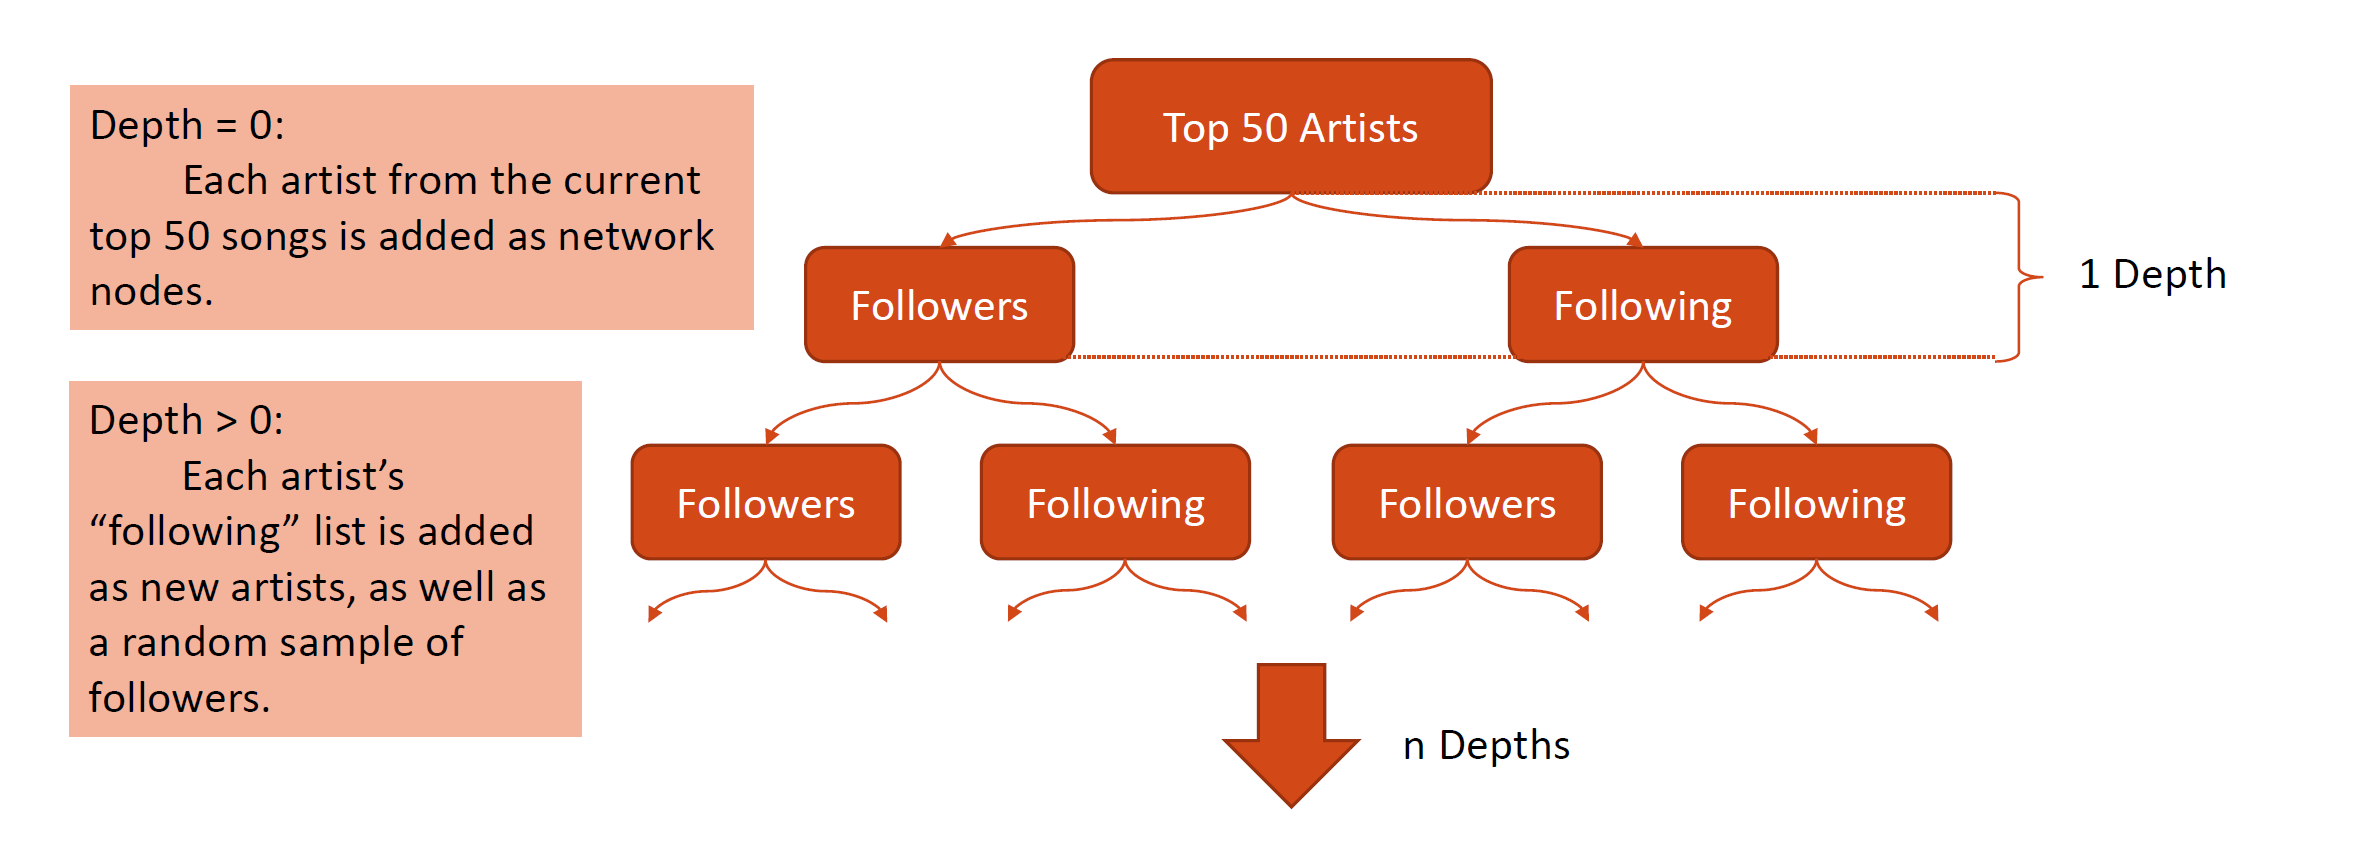
\includegraphics[scale=0.45]{sampling_visualization}
	\caption{Visualization of our first sampling technique.}
\end{figure}

We then had to decide what type of data to grab off of each of the SoundCloud users' profile pages.  There were many fields on the profile pages but a lot of the fields were optional when creating the page so some users did not have data for a particular field.  We ended up choosing five different fields labeled in Table 1.

\begin{table}[h!]
	\centering
	\begin{tabular}{||c c c||} 
		\hline
		Field & Datatype & Optional \\ [0.5ex] 
		\hline\hline
		id & int & False \\
		\hline
		href & string & False \\ 
		\hline
		num\_tracks & int & False \\
		\hline
		num\_followers & int & False \\
		\hline
		num\_following & int & False \\
		\hline
		city & string & True \\
		\hline
		latitude & float & True \\
		\hline
		longitude & float & True \\
		\hline
		followers & list & False \\
		\hline
		following & list & False \\
		\hline
	\end{tabular}
	\caption{Depiction of data scraped from each artist}
	\label{Table:1}
\end{table}

The first field was the "id" field, which was a unique integer assigned to each of the users in the dataset.  This was used to easily identify different users when we loaded them into the network.  The "href" field was a string that could be appended to a base soundcloud url in order to correctly request the HTML page from the server.  The "num\_tracks" field was the number of tracks the user had uploaded to his/her profile page.  This was either '> 0' if the user was an artist and '= 0' otherwise.  The "num\_followers" field was the number of followers a user had.  Similarly, the "num\_following" field was the number users the user was following.  The "city" field was a field that a user could enter a string into that could either represent their current place of residence or their hometown.  From the "city" field, we calculated the latitude and longitude fields.  The last two fields, "followers" and "following," were each lists containing the names of each of the other users the user was connected to.

Note that we initially chose these fields with the intent to perform link prediction on nodes in the network and predict whether an artist was about to rise quickly in popularity.  Based on issues explained in more detail in the results section, we used only a fraction of these fields in our analysis.

\subsection{Network}

After obtaining all of the data from SoundCloud and storing it into a dictionary, we needed to decide how to load it into a structure where we could perform our analysis on it. We opted to use the package NetworkX as we were very familiar with it and all of its functionality.  We made a big design decision to keep the network's edges undirected versus directed because otherwise it would limit us to be able to use certain functions in the NetworkX package as well as make it more difficult to generate a densley connected graph given our time constraints.  We knew that this network seemed to abstract better to a directed network and therefore we coded in the option to generate one in the future.

\section{Analysis}

After gathering the data to populate our network and loading it into NetworkX in order to conceptualize it, we realized very quickly that we were going to have to refine our method for sampling the data.  It was readily apparent that the graph generated was not very correlated to the structure of the full network.  Because most of the project was spent refining the sampling techniques, we decided to shift our focus from link prediction and rising artist analysis to analyzing the effect of different sampling techniques on the structure of the network generated.  In order to do so, we chose on using a consistent set of algorithms to test on the graph and consistent set of metrics to characterize the graph.  For algorithms, we chose the Guilt by Association heuristic and Link Prediction based on degree product, common neighbor, and shortest path heuristics.  For the metrics, we chose to use clustering coefficients, the total number of triangles, and degrees.  Each of these algorithms and metrics are discussed in more detail in their respected sections.

\subsection{Network Topologies}
The first network topology that we made was generated from our initial sampling design decision to snowball outwards from the "Top 50" songs chart.  We initially grabbed each of the artists on this page and then grabbed a subset of their followers and the users the artists were following.  We only grabbed a subset (initally unbeknown to us) because we ran into a large roadblock where SoundCloud had implemented an "infinite scrolling" feature on the "following" and "followers" pages attached to a profile page.  This feature loaded only twenty different artists initially when you made a request for the page until the user scrolled down to the bottom of the page, in which case twenty more artists would be loaded.  This process would be repeated until all of the followers or following were displayed.  After realizing this, we needed to implement a solution where we utilized a package called Selenium. This package implements a chrome driver to allow programmatic control over the chrome web application.  We then used javascript package called JQuery in order to send a request to the SoundCloud server to send us the next twenty users in the followers and following web pages.  We repeated this JQuery request a total of 10 times, stalling the script for a tenth of second in between to give time for the server to process the request and to account for latency.  This still only gave us a maximum of around 200 followers and 200 following.  We would've preferred to keep this script running until all of the users were loaded but we didn't due to time constraints.  Below in Figure 2 is a visual representation of our first network generated. 

\begin{figure}[h]
	\centering
	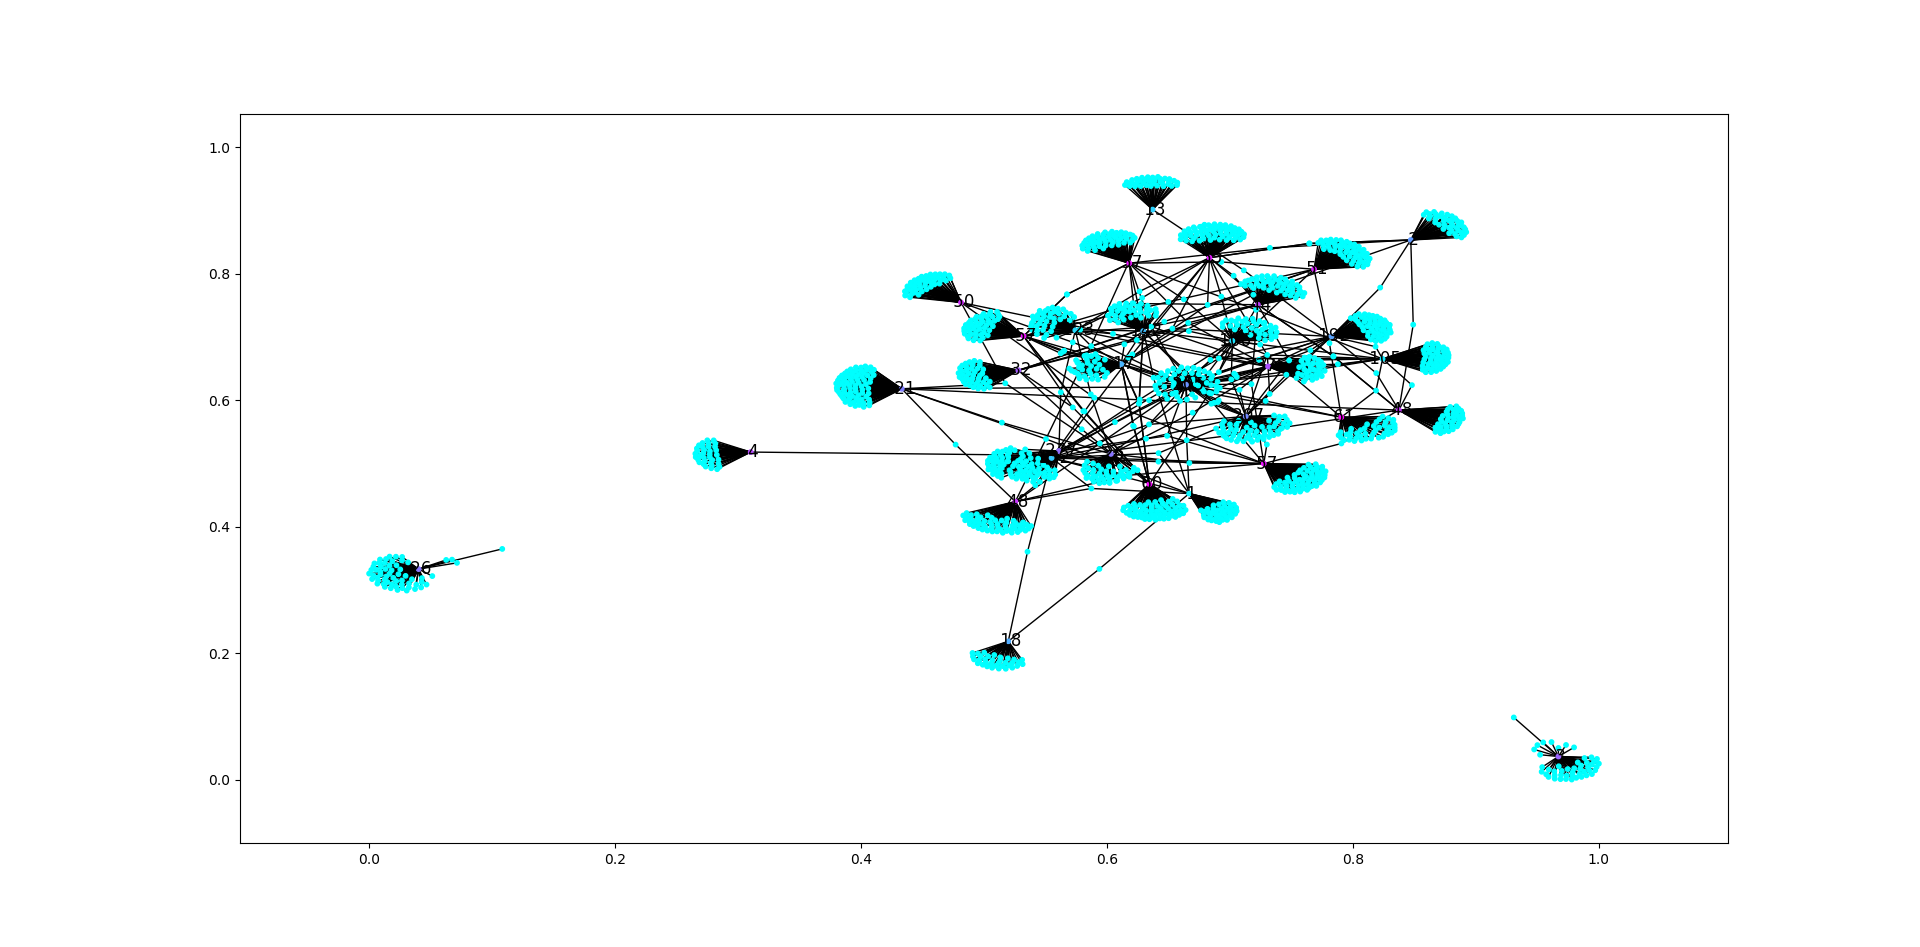
\includegraphics[scale=0.29]{take_1_visualization}
	\caption{Visualization of our first network topology.  Note that this network is scaled down to the first 500 nodes that were originally added.  The network consisted of around 21,000 nodes and 30,000 edges when we finished scraping and began to perform our algorithms and metrics on it.  The colors and numbers on the nodes are representing the number of tracks each of the users had.}
\end{figure}

The visualization of the network is exactly what we expected to see because of the sampling scheme that we used.  Each of the nodes in the visualization are colored based on the number of tracks attribute.  Thus, the cyan nodes are users that had the number of tracks attribute equal to zero.  You can see that there are many cyan nodes that fan out connections to a different colored node in the center.  These different colored nodes indicate the first 40-50 artists that we grabbed from the "Top 50" song charts seed webpage.  The cyan users indicate the followers and following of the initial artists.  There are also some cyan nodes in the middle that have multiple connections to a variety of different colored nodes.  We expected to see this because most of the "Top 50" songs were in the rap genre and therefore, we believed it would be more probable for the different artists in the "Top 50" to share different followers and following.  We did not believe that this small, subset-network was structurally similar to the full SoundCloud network.  This belief was the motivation to creating our second network topology.

The second network generated was the result of a change in our sampling technique.  We wanted the network to have more connections between nodes because we believed it would be more similar to the full network.  In order to do this, we thought we could adjust our sampling technique to adaptive sampling.  We used our initial pickled users file after our script captured the nodes and edges from "depth=1" (refer to Figure 1 for a better understanding).  We then branched out from those users to only the users they were following.  We believed this would give us a network that would contain many more artists rather than users because most artists have a larger following/followers ratio.  We were hoping this would lead us to a more connected network as well because we thought the initial followers of the "Top 50" artists would make connections to many more common artists since most of the "Top 50" artists were in the same genre.  Below is a depiction of the network generated from our second sampling technique.

\begin{figure}[h]
	\centering
	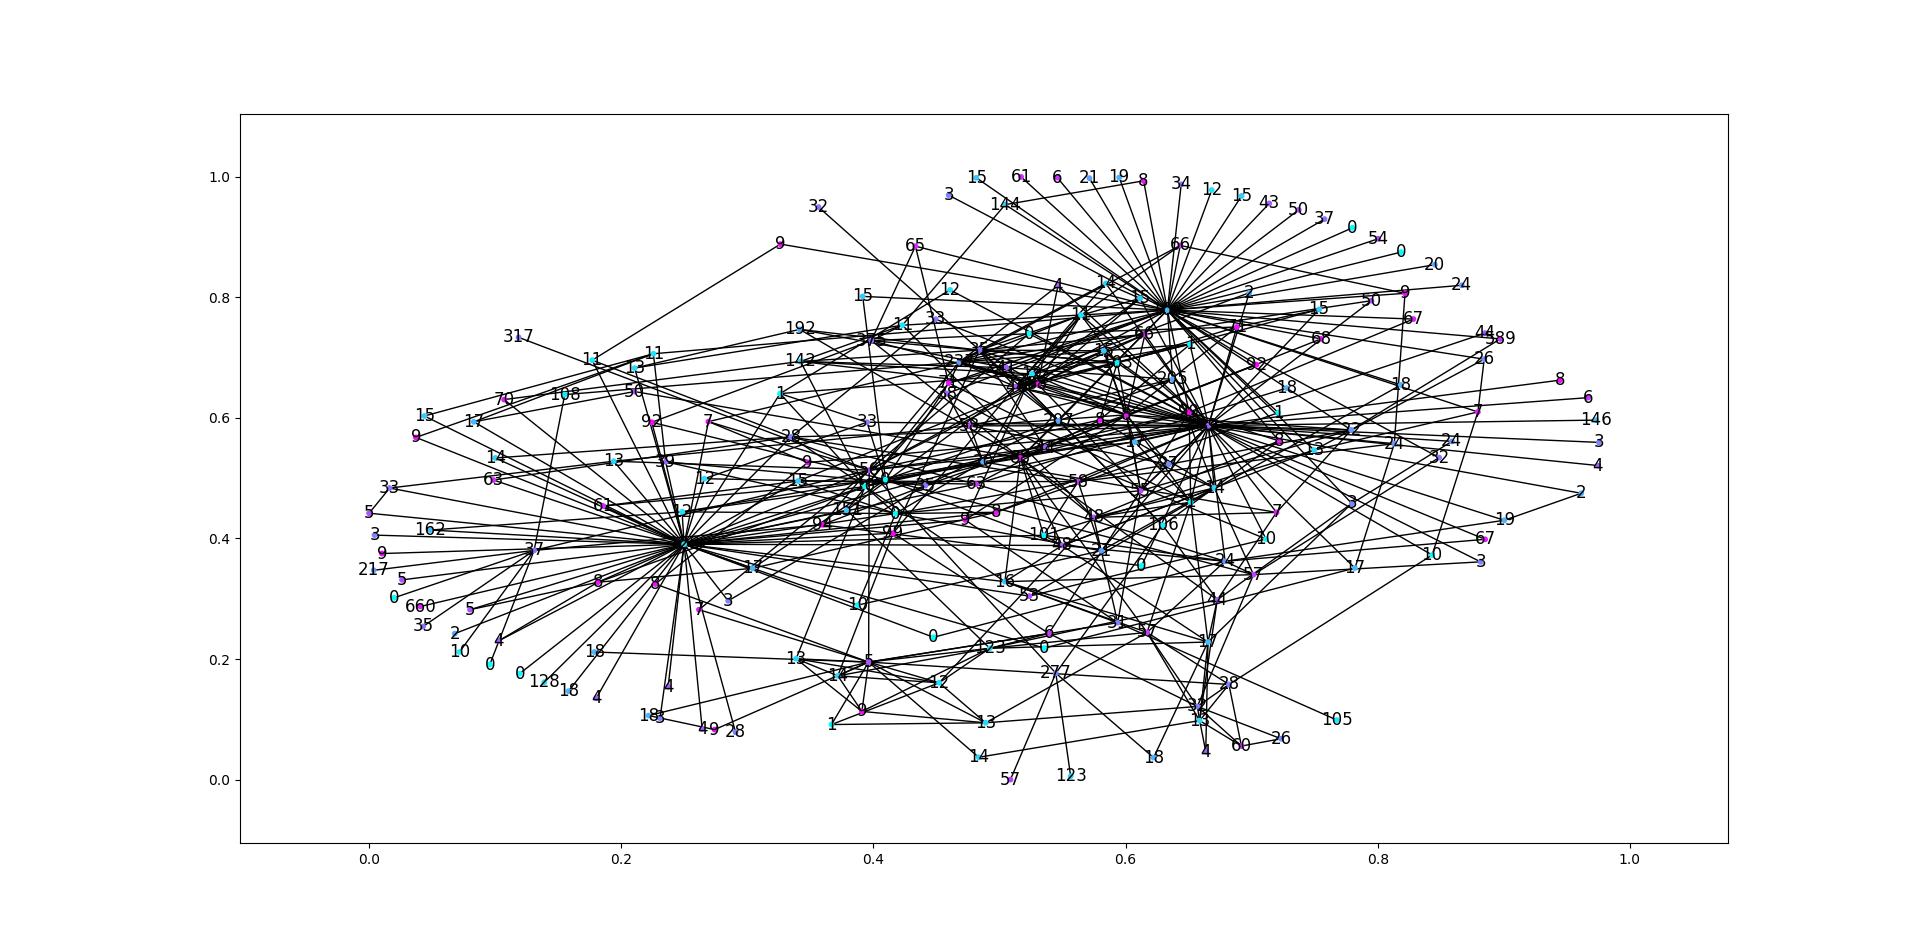
\includegraphics[scale=0.29]{take_2_visualization}
	\caption{Visualization of our second network topology.  Note that this network is scaled down using a function that removed any of the users that did not upload any tracks to the profile page (387 nodes).  The network consisted of around 40,000 nodes and 60,000 edges when we finished scraping and began to perform our algorithms and metrics on it.  The colors and numbers on the nodes are representing the number of tracks each of the users had.}
\end{figure}

While this visualization shows a very connected network, it is hard to compare this graph to the first graph.  We did not create a visualization in exactly the same manner as the first visualization because it would've given us the exact same figure.  This is because we used the pickled file of initial users from the first sampling in order to provide the seed for our second graph.  If we used this and did the same process of graphing the first 500 nodes added, they would've been identical figures.  In order to get a different visualization of the network, we made a function that "cleaned" the dataset and removed any of the users that did not upload any tracks.  We believed that this dataset would then only entail the "artists" in our dataset.  Even so, after analyzing our network we still believed the network was not very structurally similar to the full SoundCloud network so this motivated us to adjust our sampling technique even further.

For our third network, we wanted to encompass a more representative sample of all of the artists on the network and not just the artists from the rap genre.  In order to do this, we utilized the adaptive sampling technique from our second take to only grab the followers of the users from the initial seed.  We also changed our initial seed of users to contain the artists of the "Top 50" songs from each of the genres labeled on SoundCloud.  There were 30 different genres total, represented in the table below.  Each of these HTML pages were very similar to the first "Top 50" songs page where we gathered our initial seed for the first two sampling techniques, so it was quite easy to adjust our scripts in order to populate our new seed of users.  Below is a visualization of our third network generated from this new sampling technique.

\begin{figure}[h]
	\centering
	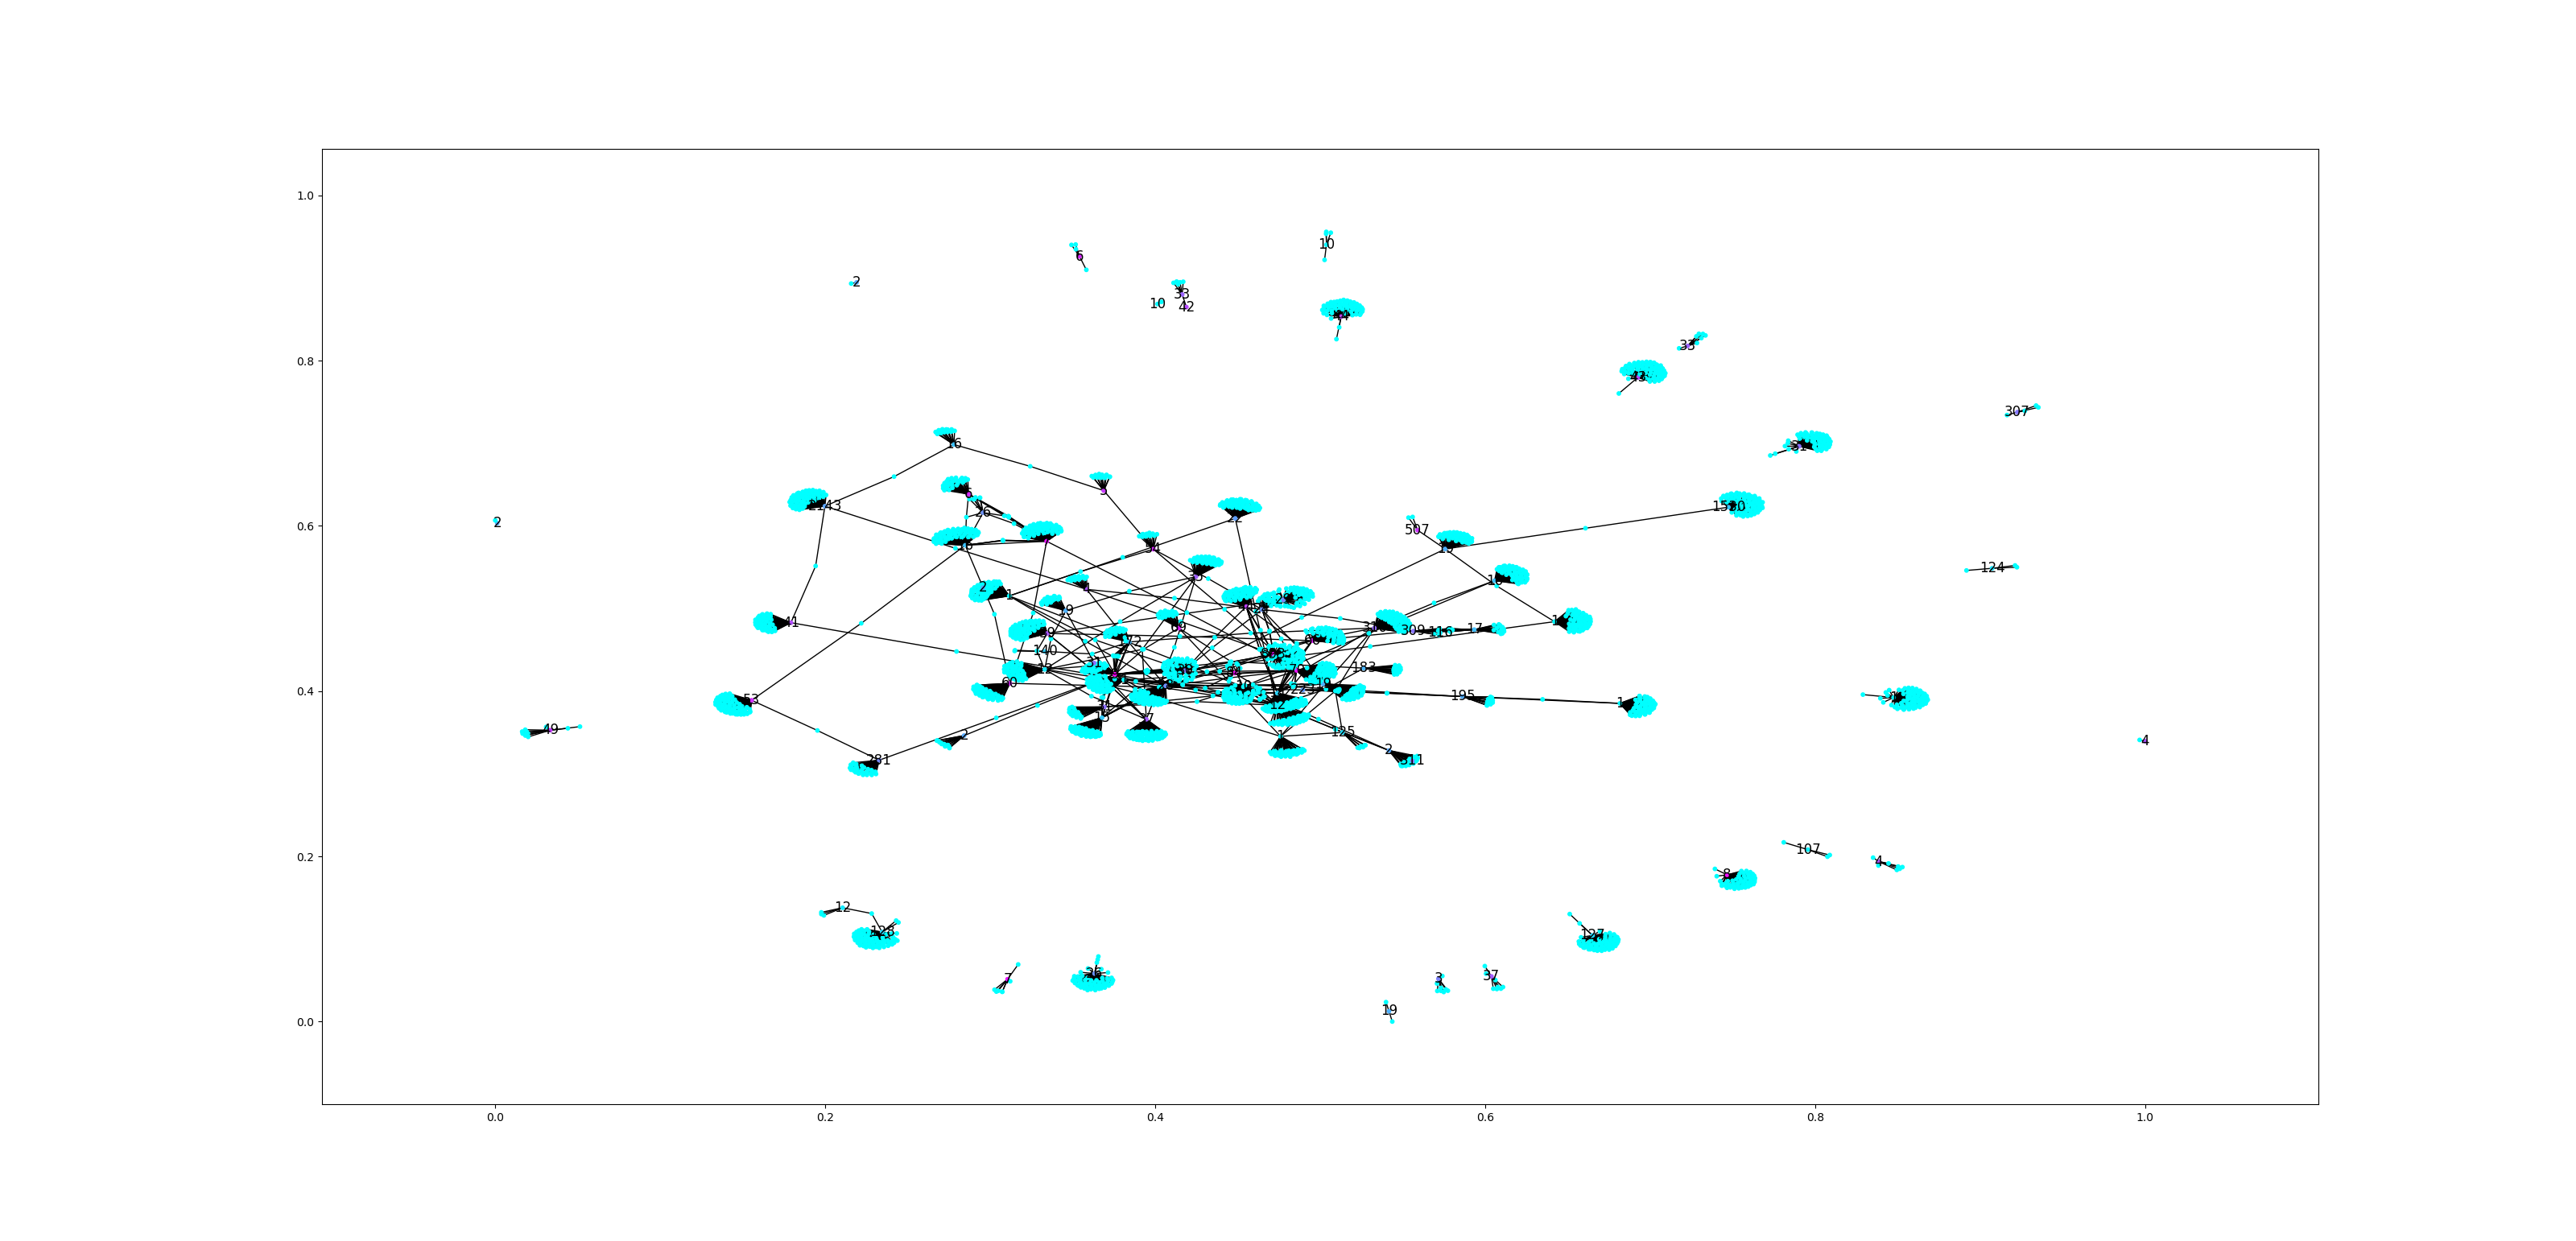
\includegraphics[scale=0.29]{take_3_visualization}
	\caption{Visualization of our third network topology.  Note that this network is scaled down to the first 500 nodes that were originally added.  The network consisted of around 6,000 nodes and 6,000 edges when we finished scraping and began to perform our algorithms and metrics on it.  The colors and numbers on the nodes are representing the number of tracks each of the users had.}
\end{figure}

In this network, we were surprised to see the number of components in the graph greatly increase from the previous network.  We believed that changing the sampling technique to only gather the users that were followed by a particular user would keep the network very connected.  Upon further investigation, we believe that the number of components is due to the different genres of music an artist is apart of.  It is reasonable to believe that there are different communities of users within that can be discerned from different genres as people tend to enjoy one or a few different genres rather than all of the genres in a given spectrum.  It is also apparent that most of the nodes in our graph represent users and not artists as the color of the majority of nodes is cyan blue (num\_tracks=0).

\section*{References}
\small

[1] Boyd, d. m. and Ellison, N. B. (2007), Social Network Sites: Definition, History, and Scholarship. Journal of Computer-Mediated Communication, 13: 210–230. doi:10.1111/j.1083-6101.2007.00393.x

[2] Clauset, A 2017, Lecture 9: Sampling, lecture notes, Network Analysis and Modeling, University of Colorado Boulder, delivered 31 October 2017


\end{document}